% Options for packages loaded elsewhere
\PassOptionsToPackage{unicode}{hyperref}
\PassOptionsToPackage{hyphens}{url}
%
\documentclass[
]{book}
\usepackage{amsmath,amssymb}
\usepackage{iftex}
\ifPDFTeX
  \usepackage[T1]{fontenc}
  \usepackage[utf8]{inputenc}
  \usepackage{textcomp} % provide euro and other symbols
\else % if luatex or xetex
  \usepackage{unicode-math} % this also loads fontspec
  \defaultfontfeatures{Scale=MatchLowercase}
  \defaultfontfeatures[\rmfamily]{Ligatures=TeX,Scale=1}
\fi
\usepackage{lmodern}
\ifPDFTeX\else
  % xetex/luatex font selection
\fi
% Use upquote if available, for straight quotes in verbatim environments
\IfFileExists{upquote.sty}{\usepackage{upquote}}{}
\IfFileExists{microtype.sty}{% use microtype if available
  \usepackage[]{microtype}
  \UseMicrotypeSet[protrusion]{basicmath} % disable protrusion for tt fonts
}{}
\makeatletter
\@ifundefined{KOMAClassName}{% if non-KOMA class
  \IfFileExists{parskip.sty}{%
    \usepackage{parskip}
  }{% else
    \setlength{\parindent}{0pt}
    \setlength{\parskip}{6pt plus 2pt minus 1pt}}
}{% if KOMA class
  \KOMAoptions{parskip=half}}
\makeatother
\usepackage{xcolor}
\usepackage{color}
\usepackage{fancyvrb}
\newcommand{\VerbBar}{|}
\newcommand{\VERB}{\Verb[commandchars=\\\{\}]}
\DefineVerbatimEnvironment{Highlighting}{Verbatim}{commandchars=\\\{\}}
% Add ',fontsize=\small' for more characters per line
\usepackage{framed}
\definecolor{shadecolor}{RGB}{248,248,248}
\newenvironment{Shaded}{\begin{snugshade}}{\end{snugshade}}
\newcommand{\AlertTok}[1]{\textcolor[rgb]{0.94,0.16,0.16}{#1}}
\newcommand{\AnnotationTok}[1]{\textcolor[rgb]{0.56,0.35,0.01}{\textbf{\textit{#1}}}}
\newcommand{\AttributeTok}[1]{\textcolor[rgb]{0.13,0.29,0.53}{#1}}
\newcommand{\BaseNTok}[1]{\textcolor[rgb]{0.00,0.00,0.81}{#1}}
\newcommand{\BuiltInTok}[1]{#1}
\newcommand{\CharTok}[1]{\textcolor[rgb]{0.31,0.60,0.02}{#1}}
\newcommand{\CommentTok}[1]{\textcolor[rgb]{0.56,0.35,0.01}{\textit{#1}}}
\newcommand{\CommentVarTok}[1]{\textcolor[rgb]{0.56,0.35,0.01}{\textbf{\textit{#1}}}}
\newcommand{\ConstantTok}[1]{\textcolor[rgb]{0.56,0.35,0.01}{#1}}
\newcommand{\ControlFlowTok}[1]{\textcolor[rgb]{0.13,0.29,0.53}{\textbf{#1}}}
\newcommand{\DataTypeTok}[1]{\textcolor[rgb]{0.13,0.29,0.53}{#1}}
\newcommand{\DecValTok}[1]{\textcolor[rgb]{0.00,0.00,0.81}{#1}}
\newcommand{\DocumentationTok}[1]{\textcolor[rgb]{0.56,0.35,0.01}{\textbf{\textit{#1}}}}
\newcommand{\ErrorTok}[1]{\textcolor[rgb]{0.64,0.00,0.00}{\textbf{#1}}}
\newcommand{\ExtensionTok}[1]{#1}
\newcommand{\FloatTok}[1]{\textcolor[rgb]{0.00,0.00,0.81}{#1}}
\newcommand{\FunctionTok}[1]{\textcolor[rgb]{0.13,0.29,0.53}{\textbf{#1}}}
\newcommand{\ImportTok}[1]{#1}
\newcommand{\InformationTok}[1]{\textcolor[rgb]{0.56,0.35,0.01}{\textbf{\textit{#1}}}}
\newcommand{\KeywordTok}[1]{\textcolor[rgb]{0.13,0.29,0.53}{\textbf{#1}}}
\newcommand{\NormalTok}[1]{#1}
\newcommand{\OperatorTok}[1]{\textcolor[rgb]{0.81,0.36,0.00}{\textbf{#1}}}
\newcommand{\OtherTok}[1]{\textcolor[rgb]{0.56,0.35,0.01}{#1}}
\newcommand{\PreprocessorTok}[1]{\textcolor[rgb]{0.56,0.35,0.01}{\textit{#1}}}
\newcommand{\RegionMarkerTok}[1]{#1}
\newcommand{\SpecialCharTok}[1]{\textcolor[rgb]{0.81,0.36,0.00}{\textbf{#1}}}
\newcommand{\SpecialStringTok}[1]{\textcolor[rgb]{0.31,0.60,0.02}{#1}}
\newcommand{\StringTok}[1]{\textcolor[rgb]{0.31,0.60,0.02}{#1}}
\newcommand{\VariableTok}[1]{\textcolor[rgb]{0.00,0.00,0.00}{#1}}
\newcommand{\VerbatimStringTok}[1]{\textcolor[rgb]{0.31,0.60,0.02}{#1}}
\newcommand{\WarningTok}[1]{\textcolor[rgb]{0.56,0.35,0.01}{\textbf{\textit{#1}}}}
\usepackage{longtable,booktabs,array}
\usepackage{calc} % for calculating minipage widths
% Correct order of tables after \paragraph or \subparagraph
\usepackage{etoolbox}
\makeatletter
\patchcmd\longtable{\par}{\if@noskipsec\mbox{}\fi\par}{}{}
\makeatother
% Allow footnotes in longtable head/foot
\IfFileExists{footnotehyper.sty}{\usepackage{footnotehyper}}{\usepackage{footnote}}
\makesavenoteenv{longtable}
\usepackage{graphicx}
\makeatletter
\def\maxwidth{\ifdim\Gin@nat@width>\linewidth\linewidth\else\Gin@nat@width\fi}
\def\maxheight{\ifdim\Gin@nat@height>\textheight\textheight\else\Gin@nat@height\fi}
\makeatother
% Scale images if necessary, so that they will not overflow the page
% margins by default, and it is still possible to overwrite the defaults
% using explicit options in \includegraphics[width, height, ...]{}
\setkeys{Gin}{width=\maxwidth,height=\maxheight,keepaspectratio}
% Set default figure placement to htbp
\makeatletter
\def\fps@figure{htbp}
\makeatother
\setlength{\emergencystretch}{3em} % prevent overfull lines
\providecommand{\tightlist}{%
  \setlength{\itemsep}{0pt}\setlength{\parskip}{0pt}}
\setcounter{secnumdepth}{5}
\usepackage{booktabs}
\ifLuaTeX
  \usepackage{selnolig}  % disable illegal ligatures
\fi
\usepackage[]{natbib}
\bibliographystyle{plainnat}
\usepackage{bookmark}
\IfFileExists{xurl.sty}{\usepackage{xurl}}{} % add URL line breaks if available
\urlstyle{same}
\hypersetup{
  pdftitle={Bookdown: Flexible Document Creation in RStudio},
  pdfauthor={Joseph Thiers},
  hidelinks,
  pdfcreator={LaTeX via pandoc}}

\title{Bookdown: Flexible Document Creation in RStudio}
\author{Joseph Thiers}
\date{}

\usepackage{amsthm}
\newtheorem{theorem}{Theorem}[chapter]
\newtheorem{lemma}{Lemma}[chapter]
\newtheorem{corollary}{Corollary}[chapter]
\newtheorem{proposition}{Proposition}[chapter]
\newtheorem{conjecture}{Conjecture}[chapter]
\theoremstyle{definition}
\newtheorem{definition}{Definition}[chapter]
\theoremstyle{definition}
\newtheorem{example}{Example}[chapter]
\theoremstyle{definition}
\newtheorem{exercise}{Exercise}[chapter]
\theoremstyle{definition}
\newtheorem{hypothesis}{Hypothesis}[chapter]
\theoremstyle{remark}
\newtheorem*{remark}{Remark}
\newtheorem*{solution}{Solution}
\begin{document}
\maketitle

{
\setcounter{tocdepth}{1}
\tableofcontents
}
\chapter{Introduction to RStudio and Bookdown}\label{introduction-to-rstudio-and-bookdown}

Welcome to this \textbf{Bookdown tutorial} a guide created to introduce students, researchers, and professionals to flexible document creation within RStudio using the \texttt{bookdown} package. Bookdown is ideal for creating single-page assignments, reports, academic papers, and even full-length books that combine text, code, and visualizations.

\section{Why RStudio and Bookdown?}\label{why-rstudio-and-bookdown}

Bookdown within RStudio supports dynamic, reproducible, and structured document creation. This is especially useful for students and professionals in mathematics where equations, figures, and analysis are integral to the work. While tools like LaTeX, Microsoft Word, or PowerPoint each have their strengths, Bookdown brings the unique ability to integrate text, code, data analysis, and figures in one streamlined, reproducible workflow.

\section{What You'll Learn in This Tutorial}\label{what-youll-learn-in-this-tutorial}

This tutorial covers the essential aspects of using Bookdown:

\begin{itemize}
\item
  \textbf{Chapter 1}: Setting Up Bookdown -- Installing the package and configuring a Bookdown project in RStudio.
\item
  \textbf{Chapter 2}: Writing and Structuring Content -- Using R Markdown syntax to create chapters, add code chunks, cross-references, and other essentials.
\item
  \textbf{Chapter 3}: Customizing Output -- Exporting your book in HTML, PDF, or EPUB, along with tips on styling and configuration.
\item
  \textbf{Chapter 4}: Advanced Features and Practical Example -- Integrating citations, managing references, and a full walkthrough using a real paper example.
\end{itemize}

\section{Getting Started}\label{getting-started}

To get started with this tutorial please follow these steps:

\begin{enumerate}
\def\labelenumi{\arabic{enumi}.}
\tightlist
\item
  \textbf{Install R}:
  Go to the \href{https://cran.r-project.org/}{R Project download page} and download the latest version of R for your operating system (Windows, macOS, or Linux). Follow the installation instructions provided.
\end{enumerate}


\includegraphics{images/tutorialscreenshots/installR.png}

\begin{enumerate}
\def\labelenumi{\arabic{enumi}.}
\setcounter{enumi}{1}
\tightlist
\item
  \textbf{Install RStudio}:
  Go to the \href{https://posit.co/download/rstudio-desktop/}{RStudio download page} and select the appropriate version for your operating system (Windows, macOS, or Linux). Download and follow the installation instructions.
\end{enumerate}


\includegraphics{images/tutorialscreenshots/installRStudio.png}

\begin{enumerate}
\def\labelenumi{\arabic{enumi}.}
\setcounter{enumi}{2}
\tightlist
\item
  \textbf{Install Bookdown}:
  Once RStudio is installed next install the Bookdown package. You can do this by typing the following code into the RStudio console:
\end{enumerate}

\begin{verbatim}
install.packages("bookdown")
\end{verbatim}

You can also install the Bookdown package by:

\begin{enumerate}
\def\labelenumi{\roman{enumi}.}
\item
  Select Packages in the bottom right-hand side of RStudio
  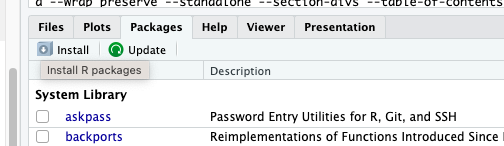
\includegraphics{images/tutorialscreenshots/installPackage.png}
\item
  Select Install
\item
  Enter bookdown under Packages
\end{enumerate}

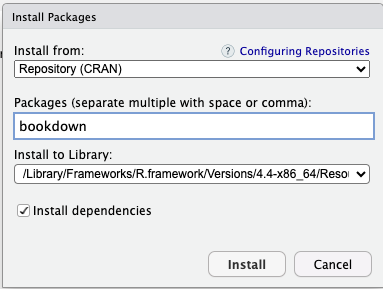
\includegraphics{images/tutorialscreenshots/installBookdownPack.png}

\begin{enumerate}
\def\labelenumi{\roman{enumi}.}
\setcounter{enumi}{3}
\tightlist
\item
  Click Install
\end{enumerate}

\begin{enumerate}
\def\labelenumi{\arabic{enumi}.}
\setcounter{enumi}{3}
\tightlist
\item
  \textbf{Create a new Bookdown Project within RStudio}
\end{enumerate}

\begin{itemize}
\tightlist
\item
  In RStudio go to \textbf{File \textgreater{} New Project}
\item
  Now select \textbf{New Project} then under the listed project types select \textbf{Book Project using Bookdown}.
\item
  Name your project and choose a location to save the new Bookdown project to.
\end{itemize}

\begin{enumerate}
\def\labelenumi{\arabic{enumi}.}
\setcounter{enumi}{4}
\tightlist
\item
  \textbf{Render Your Newly Created Book}
  In the \textbf{Build} pane:
\end{enumerate}

\begin{itemize}
\tightlist
\item
  Select \textbf{Build Book} and choose your output format, or select \emph{All formats} to render your files as HTML, pdf, and epub using the default settings.
\item
  You can also render the book directly from the R console with the following command:
\end{itemize}

\begin{verbatim}
bookdown::render_book("index.Rmd")
\end{verbatim}

\chapter{Writing and Structuring Content}\label{writing-and-structuring-content}

In this chapter, we will explore how to write and structure content in Bookdown using R Markdown syntax. Bookdown allows you to create well-organized documents by combining text, code, and references. Here, we'll cover the essentials for writing chapters, adding code chunks, creating cross-references, and structuring your content.

\section{Creating Chapters and Sections}\label{creatingchapters}

Each chapter in Bookdown is represented by a separate \texttt{.Rmd} file, and each \texttt{.Rmd} file should begin with a first-level heading, marked by a single \texttt{\#} symbol. For example:

\begin{Shaded}
\begin{Highlighting}[]
\FunctionTok{\# Chapter Title}
\end{Highlighting}
\end{Shaded}

Chapters are automatically numbered based on their order in the project directory, so make sure each file name reflects its chapter number (e.g., 02-writing-structuring-content.Rmd for Chapter 2).

\section{Adding Sections and Subsections}\label{adding-sections-and-subsections}

You can add sections and subsections within a chapter using second-level and higher-level headings:

\begin{verbatim}
## Section Title
### Subsection Title
\end{verbatim}

This hierarchy of sections and subsections organizes the document and they will automatically appear in the table of contents.

Adding Code Chunks

One of the strengths of Bookdown is the ability to incorporate live R code into your document. Code chunks in R Markdown are written between three backticks (```) with \{r\} specifying R as the language:

\begin{Shaded}
\begin{Highlighting}[]
\CommentTok{\# R code example}
\FunctionTok{summary}\NormalTok{(cars)}
\end{Highlighting}
\end{Shaded}

\begin{verbatim}
##      speed           dist       
##  Min.   : 4.0   Min.   :  2.00  
##  1st Qu.:12.0   1st Qu.: 26.00  
##  Median :15.0   Median : 36.00  
##  Mean   :15.4   Mean   : 42.98  
##  3rd Qu.:19.0   3rd Qu.: 56.00  
##  Max.   :25.0   Max.   :120.00
\end{verbatim}

\subsection{Customizing Code Chunk Options}\label{customizing-code-chunk-options}

You can customize how code chunks appear using chunk options. Here are a few common options:

\begin{itemize}
\tightlist
\item
  \textbf{\texttt{echo=FALSE}}: Hides the code but displays the output.
\item
  \textbf{\texttt{eval=FALSE}}: Shows the code but does not execute it.
\item
  \textbf{\texttt{fig.cap="Caption\ Text"}}: Adds a caption to figures generated from the code chunk.
\item
  \textbf{\texttt{out.width="50\%"}}: Sets the output width for images generated in the chunk.
\end{itemize}

Example:

\begin{Shaded}
\begin{Highlighting}[]
\FunctionTok{summary}\NormalTok{(cars)}
\end{Highlighting}
\end{Shaded}

\begin{verbatim}
##      speed           dist       
##  Min.   : 4.0   Min.   :  2.00  
##  1st Qu.:12.0   1st Qu.: 26.00  
##  Median :15.0   Median : 36.00  
##  Mean   :15.4   Mean   : 42.98  
##  3rd Qu.:19.0   3rd Qu.: 56.00  
##  Max.   :25.0   Max.   :120.00
\end{verbatim}

Experiment with these options to control how your code and output appear.

\section{Cross-Referencing Sections, Figures, and Tables}\label{cross-referencing-sections-figures-and-tables}

Bookdown makes it easy to create cross-references for sections, figures, and tables.

\subsection{Cross-Referencing Sections}\label{cross-referencing-sections}

To reference a section, add an ID to the heading by including \texttt{\{\#your-id\}} at the end:

\begin{Shaded}
\begin{Highlighting}[]
\FunctionTok{\#\# Creating Chapters and Sections \{\#creatingchapters\}}
\end{Highlighting}
\end{Shaded}

Then, refer to it later in your document with

\begin{Shaded}
\begin{Highlighting}[]
\NormalTok{\textbackslash{}@ref():}
\end{Highlighting}
\end{Shaded}

As we can see here by referring back to section 2.1 Creating Chapters and Sections
Watch us go right back to Section \ref{creatingchapters},

\begin{Shaded}
\begin{Highlighting}[]
\NormalTok{\textbackslash{}@ref(creatingchapters)}
\end{Highlighting}
\end{Shaded}

\section{Cross-Referencing Figures GO BACK ANMD CHANGE FIX}\label{cross-referencing-figures-go-back-anmd-change-fix}

For figures, use the fig.cap option to create a caption and \texttt{\textbackslash{}@ref(fig:label)} to reference it:

\begin{Shaded}
\begin{Highlighting}[]
\FunctionTok{plot}\NormalTok{(cars}\SpecialCharTok{$}\NormalTok{speed, cars}\SpecialCharTok{$}\NormalTok{dist)}
\end{Highlighting}
\end{Shaded}

\begin{figure}

{\centering 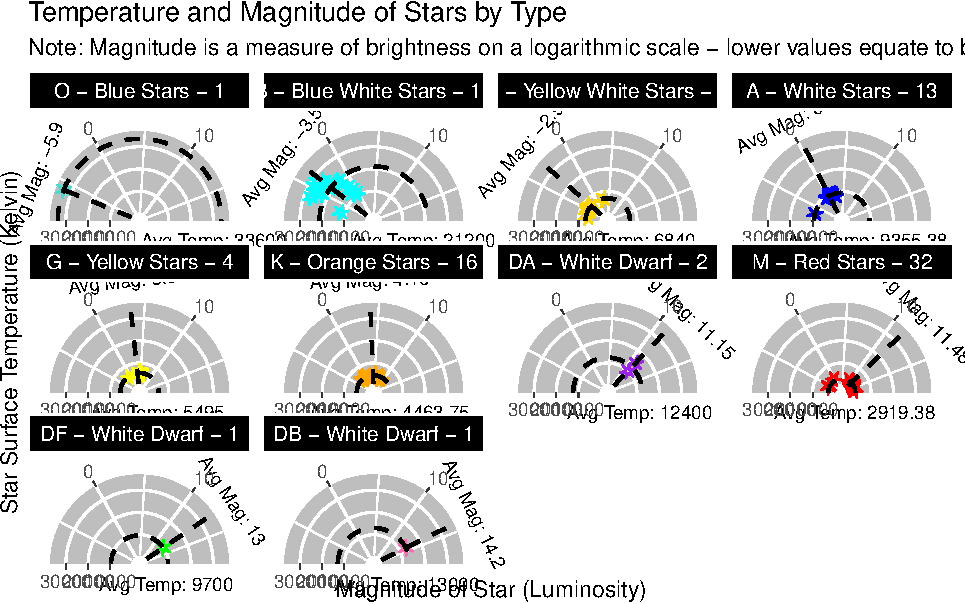
\includegraphics{_main_files/figure-latex/unnamed-chunk-7-1} 

}

\caption{A scatter plot of speed vs. distance}\label{fig:unnamed-chunk-7}
\end{figure}

Refer to Figure \citet{ref}(``A scatter plot of speed vs.~distance'') to see the plot.

\subsection{Cross-Referencing Tables}\label{cross-referencing-tables}

To reference tables, you can use the \texttt{knitr::kable()} function to create a table and set a label:

\begin{Shaded}
\begin{Highlighting}[]
\NormalTok{knitr}\SpecialCharTok{::}\FunctionTok{kable}\NormalTok{(}\FunctionTok{head}\NormalTok{(cars), }\AttributeTok{caption =} \StringTok{"Table of the first rows of the cars dataset"}\NormalTok{)}
\end{Highlighting}
\end{Shaded}

\begin{table}

\caption{(\#tab:tab:cars-table)Table of the first rows of the cars dataset}
\centering
\begin{tabular}[t]{r|r}
\hline
speed & dist\\
\hline
4 & 2\\
\hline
4 & 10\\
\hline
7 & 4\\
\hline
7 & 22\\
\hline
8 & 16\\
\hline
9 & 10\\
\hline
\end{tabular}
\end{table}

You can then reference it as Table \citet{ref}(tab).

\section{Formatting Text in Bookdown}\label{formatting-text-in-bookdown}

Bookdown supports a wide range of Markdown formatting. Here are a few basics:

\begin{itemize}
\item
  Bold: \texttt{**bold\ text**} -\textgreater{} \textbf{bold text}
\item
  Italics: \texttt{*italicized\ text*} -\textgreater{} \emph{italicized text}
\item
  Bullet Points:
  -First item
  -Second item
\item
  Numbered Lists:
\end{itemize}

\begin{enumerate}
\def\labelenumi{\arabic{enumi}.}
\tightlist
\item
  First item

  \begin{enumerate}
  \def\labelenumii{\roman{enumii}.}
  \tightlist
  \item
    Even sublists
  \item
    Like this
  \end{enumerate}
\item
  Second item
\end{enumerate}

Use these formatting options to style text and create lists within your chapters.
Conclusion

In this chapter, we covered the basics of structuring a Bookdown document. You learned how to create chapters and sections, add code chunks, and use cross-references for figures, tables, and sections. Structuring your content well will help readers navigate your document and make your analysis easier to follow.

Continue to the next chapter to learn how to customize the appearance and output format of your Bookdown project.

\chapter{Cross-references}\label{cross}

Cross-references make it easier for your readers to find and link to elements in your book.

\section{Chapters and sub-chapters}\label{chapters-and-sub-chapters}

There are two steps to cross-reference any heading:

\begin{enumerate}
\def\labelenumi{\arabic{enumi}.}
\tightlist
\item
  Label the heading: \texttt{\#\ Hello\ world\ \{\#nice-label\}}.

  \begin{itemize}
  \tightlist
  \item
    Leave the label off if you like the automated heading generated based on your heading title: for example, \texttt{\#\ Hello\ world} = \texttt{\#\ Hello\ world\ \{\#hello-world\}}.
  \item
    To label an un-numbered heading, use: \texttt{\#\ Hello\ world\ \{-\#nice-label\}} or \texttt{\{\#\ Hello\ world\ .unnumbered\}}.
  \end{itemize}
\item
  Next, reference the labeled heading anywhere in the text using \texttt{\textbackslash{}@ref(nice-label)}; for example, please see Chapter \ref{cross}.

  \begin{itemize}
  \tightlist
  \item
    If you prefer text as the link instead of a numbered reference use: \hyperref[cross]{any text you want can go here}.
  \end{itemize}
\end{enumerate}

\section{Captioned figures and tables}\label{captioned-figures-and-tables}

Figures and tables \emph{with captions} can also be cross-referenced from elsewhere in your book using \texttt{\textbackslash{}@ref(fig:chunk-label)} and \texttt{\textbackslash{}@ref(tab:chunk-label)}, respectively.

See Figure \ref{fig:nice-fig}.

\begin{Shaded}
\begin{Highlighting}[]
\FunctionTok{par}\NormalTok{(}\AttributeTok{mar =} \FunctionTok{c}\NormalTok{(}\DecValTok{4}\NormalTok{, }\DecValTok{4}\NormalTok{, .}\DecValTok{1}\NormalTok{, .}\DecValTok{1}\NormalTok{))}
\FunctionTok{plot}\NormalTok{(pressure, }\AttributeTok{type =} \StringTok{\textquotesingle{}b\textquotesingle{}}\NormalTok{, }\AttributeTok{pch =} \DecValTok{19}\NormalTok{)}
\end{Highlighting}
\end{Shaded}

\begin{figure}

{\centering 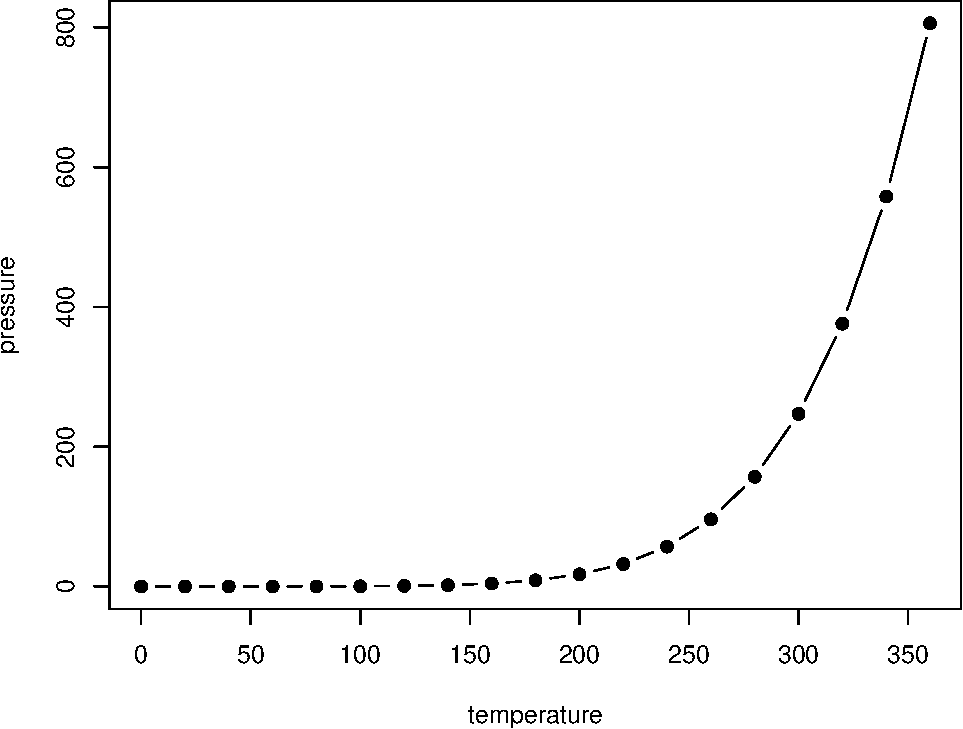
\includegraphics[width=0.8\linewidth]{_main_files/figure-latex/nice-fig-1} 

}

\caption{Here is a nice figure!}\label{fig:nice-fig}
\end{figure}

Don't miss Table \ref{tab:nice-tab}.

\begin{Shaded}
\begin{Highlighting}[]
\NormalTok{knitr}\SpecialCharTok{::}\FunctionTok{kable}\NormalTok{(}
  \FunctionTok{head}\NormalTok{(pressure, }\DecValTok{10}\NormalTok{), }\AttributeTok{caption =} \StringTok{\textquotesingle{}Here is a nice table!\textquotesingle{}}\NormalTok{,}
  \AttributeTok{booktabs =} \ConstantTok{TRUE}
\NormalTok{)}
\end{Highlighting}
\end{Shaded}

\begin{table}

\caption{\label{tab:nice-tab}Here is a nice table!}
\centering
\begin{tabular}[t]{rr}
\toprule
temperature & pressure\\
\midrule
0 & 0.0002\\
20 & 0.0012\\
40 & 0.0060\\
60 & 0.0300\\
80 & 0.0900\\
\addlinespace
100 & 0.2700\\
120 & 0.7500\\
140 & 1.8500\\
160 & 4.2000\\
180 & 8.8000\\
\bottomrule
\end{tabular}
\end{table}

\chapter{Parts}\label{parts}

You can add parts to organize one or more book chapters together. Parts can be inserted at the top of an .Rmd file, before the first-level chapter heading in that same file.

Add a numbered part: \texttt{\#\ (PART)\ Act\ one\ \{-\}} (followed by \texttt{\#\ A\ chapter})

Add an unnumbered part: \texttt{\#\ (PART\textbackslash{}*)\ Act\ one\ \{-\}} (followed by \texttt{\#\ A\ chapter})

Add an appendix as a special kind of un-numbered part: \texttt{\#\ (APPENDIX)\ Other\ stuff\ \{-\}} (followed by \texttt{\#\ A\ chapter}). Chapters in an appendix are prepended with letters instead of numbers.

\chapter{Footnotes and citations}\label{footnotes-and-citations}

\section{Footnotes}\label{footnotes}

Footnotes are put inside the square brackets after a caret \texttt{\^{}{[}{]}}. Like this one \footnote{This is a footnote.}.

\section{Citations}\label{citations}

Reference items in your bibliography file(s) using \texttt{@key}.

For example, we are using the \textbf{bookdown} package \citep{R-bookdown} (check out the last code chunk in index.Rmd to see how this citation key was added) in this sample book, which was built on top of R Markdown and \textbf{knitr} \citep{xie2015} (this citation was added manually in an external file book.bib).
Note that the \texttt{.bib} files need to be listed in the index.Rmd with the YAML \texttt{bibliography} key.

The RStudio Visual Markdown Editor can also make it easier to insert citations: \url{https://rstudio.github.io/visual-markdown-editing/\#/citations}

\chapter{Blocks}\label{blocks}

\section{Equations}\label{equations}

Here is an equation.

\begin{equation} 
  f\left(k\right) = \binom{n}{k} p^k\left(1-p\right)^{n-k}
  \label{eq:binom}
\end{equation}

You may refer to using \texttt{\textbackslash{}@ref(eq:binom)}, like see Equation \eqref{eq:binom}.

\section{Theorems and proofs}\label{theorems-and-proofs}

Labeled theorems can be referenced in text using \texttt{\textbackslash{}@ref(thm:tri)}, for example, check out this smart theorem \ref{thm:tri}.

\begin{theorem}
\protect\hypertarget{thm:tri}{}\label{thm:tri}For a right triangle, if \(c\) denotes the \emph{length} of the hypotenuse
and \(a\) and \(b\) denote the lengths of the \textbf{other} two sides, we have
\[a^2 + b^2 = c^2\]
\end{theorem}

Read more here \url{https://bookdown.org/yihui/bookdown/markdown-extensions-by-bookdown.html}.

\section{Callout blocks}\label{callout-blocks}

The R Markdown Cookbook provides more help on how to use custom blocks to design your own callouts: \url{https://bookdown.org/yihui/rmarkdown-cookbook/custom-blocks.html}

\chapter{Sharing your book}\label{sharing-your-book}

\section{Publishing}\label{publishing}

HTML books can be published online, see: \url{https://bookdown.org/yihui/bookdown/publishing.html}

\section{404 pages}\label{pages}

By default, users will be directed to a 404 page if they try to access a webpage that cannot be found. If you'd like to customize your 404 page instead of using the default, you may add either a \texttt{\_404.Rmd} or \texttt{\_404.md} file to your project root and use code and/or Markdown syntax.

\section{Metadata for sharing}\label{metadata-for-sharing}

Bookdown HTML books will provide HTML metadata for social sharing on platforms like Twitter, Facebook, and LinkedIn, using information you provide in the \texttt{index.Rmd} YAML. To setup, set the \texttt{url} for your book and the path to your \texttt{cover-image} file. Your book's \texttt{title} and \texttt{description} are also used.

This \texttt{gitbook} uses the same social sharing data across all chapters in your book- all links shared will look the same.

Specify your book's source repository on GitHub using the \texttt{edit} key under the configuration options in the \texttt{\_output.yml} file, which allows users to suggest an edit by linking to a chapter's source file.

Read more about the features of this output format here:

\url{https://pkgs.rstudio.com/bookdown/reference/gitbook.html}

Or use:

\begin{Shaded}
\begin{Highlighting}[]
\NormalTok{?bookdown}\SpecialCharTok{::}\NormalTok{gitbook}
\end{Highlighting}
\end{Shaded}

\chapter{Drought in California}\label{drought-in-california}

\section{Introduction}\label{introduction}

Droughts in California are a critical environmental issue that affects the state's water availability, agricultural sectors, and overall economy. California is known for its agricultural products and growing population, but it is also known for frequent droughts that have severely impacted the state's water resources. With the effects of climate change continuing to alter global weather patterns, droughts in the state are becoming more frequent and intense. These changes not only threaten the stability of California's agriculture but also jeopardize the water supply for millions of residents, leading to severe economic and environmental consequences. Additionally, droughts increase the risk of wildfires, which can cause widespread destruction and further strain water resources. In order to better understand drought in California, this chapter will explore the phenomenon of drought by focusing on its causes, socioeconomic impacts, effects on wildfires, the links between climate change and drought, and potential mitigation strategies.

\section{Types of Droughts}\label{types-of-droughts}

Droughts occur when there is a prolonged period of inadequate rainfall, resulting in a water shortage that impacts agricultural water supplies, municipal water systems, and natural ecosystems. Several types of droughts affect different aspects of the environment and society:

\begin{itemize}
\tightlist
\item
  \textbf{Meteorological drought}: A deficiency in precipitation over a specific period, often measured against long-term regional averages, and typically the first indicator of drought conditions.
\item
  \textbf{Agricultural drought}: Occurs when insufficient soil moisture affects crop growth and yields, threatening food production and farming livelihoods.
\item
  \textbf{Hydrological drought}: Involves the depletion of water resources in rivers, lakes, reservoirs, and groundwater systems, often following extended meteorological drought periods, with significant consequences for irrigation, drinking water supplies, and industrial uses.
\item
  \textbf{Socioeconomic drought}: Arises when the demand for water exceeds the available supply, leading to economic disruptions, particularly in water-dependent sectors like agriculture and energy.
\item
  \textbf{Ecological drought}: Impacts ecosystem health, resulting in biodiversity loss, habitat disruption, and changes in ecosystem functions due to prolonged water shortages.
\end{itemize}

In recent years, flash droughts, where conditions rapidly worsen due to rising temperatures, have become more frequent as a result of global climate change \citep{walker2023}.

\section{Causes of Drought in California}\label{causes-of-drought-in-california}

The causes of drought in California are multifaceted, involving both natural and anthropogenic factors. One primary natural cause is Pacific Sea surface temperature anomalies, which lead to persistent high-pressure systems that block rainstorms from reaching the state. This phenomenon disrupts atmospheric circulation and reduces precipitation across California, creating prolonged dry periods \citep{wei2016}. However, human-induced climate change has also significantly contributed to the severity of these droughts. Between 2012 and 2014, anthropogenic warming was estimated to account for 8-27\% of the drought conditions experienced in California, exacerbating the natural variability of drought patterns in the region \citep{williams2015}. This combination of natural variability and human-induced changes has not only increased the frequency, length, and intensity of droughts but has also strained the state's water infrastructure.

\section{Socioeconomic Impacts}\label{socioeconomic-impacts}

The socio-economic impacts of drought in California are profound. California's agricultural industry is highly dependent on easily available water, but during periods of drought, it suffers significant losses. For instance, the 2015 drought led to a reduction of 2.6 million acre-feet in water supply and an economic loss of \$1.8 billion. This caused approximately 564,000 acres of farmland to be fallowed, directly impacting agricultural revenues and employment \citep{sumner2015}. The drought also highlighted inequalities in water access, with rural communities in agricultural regions, such as Tulare County, being disproportionately affected. These communities experienced domestic well failures, emphasizing the social aspect of water scarcity in the state \citep{pompeii2020}. Environmental impacts are another significant concern, as droughts increase wildfire risks and degrade ecosystems dependent on adequate water supplies. Reduced water levels in rivers, lakes, and reservoirs also threaten fish and aquatic populations, leading to long-term ecological consequences.

\section{Wildfire Risk}\label{wildfire-risk}

One of the most significant effects of prolonged drought in California is the increased frequency and intensity of wildfires. Droughts create dry conditions, causing vegetation like grasses and trees to lose moisture and become more flammable. Without adequate rainfall, even typically fire-resistant plants dry out, providing fuel for wildfires. According to \citet{westerling2019}, a significant portion of forest fires in the western United States can be linked to drought, which has extended fire seasons and increased the areas burned. Drought-induced wildfires have devastating effects on both the environment and human communities. They destroy homes, displace residents, and damage ecosystems while also leading to carbon emissions from burning vegetation \citep{abatzoglou2016}.

\section{Climate Change and Drought}\label{climate-change-and-drought}

Climate change is a major driver of the increasing frequency and severity of droughts in California. As global temperatures continue to rise, so do evaporation rates, which reduces available surface water and soil moisture. This exacerbates the conditions that cause droughts, worsening their impacts on agriculture, water resources, and ecosystems. The 2013-2014 drought in California was partially attributed to climate change, which intensified the effects of naturally occurring weather patterns, like high-pressure systems that block rainfall \citep{mao2015}.

\section{Mitigation Strategies}\label{mitigation-strategies}

California has implemented a range of strategies to mitigate the impacts of drought, focusing on both immediate responses and long-term solutions. Water conservation, wastewater recycling, and water transfers are among the most commonly used methods. Conservation efforts, such as public water-use restrictions and the promotion of water-efficient technologies in households and agriculture, play a significant role in reducing water demand during drought periods. Wastewater recycling, in particular, has been gaining traction as a long-term solution, although it continues to face political and public resistance \citep{keavney2022}. Water transfers, which involve reallocating water from one region to another, provide flexibility in water management, helping to address shortages where they are most acute. Replenishing groundwater aquifers is another critical strategy, as aquifer depletion during droughts can lead to long-term water scarcity. Managed aquifer recharge (MAR) initiatives, which involve intentionally refilling underground aquifers during wet periods, are increasingly recognized as a sustainable way to bolster water supplies for future droughts. During the 2012-2016 drought, ranchers in California adapted by employing more proactive drought management practices, such as drip irrigation and efficient water delivery systems, which were shaped by their past experiences with severe droughts \citep{woodmansee2021}.

\section{Conclusion}\label{conclusion}

Drought in California represents a vast and complex challenge that affects all aspects of life in the state, from agriculture to urban water supplies. The causes of drought are both natural and human-induced, showing a need for a comprehensive approach in addressing it. Climate change continues to play a critical role in exacerbating drought conditions, while the socio-economic impacts of drought are severe, particularly in rural agricultural communities and ecosystems that depend on reliable water supplies. Moving forward, a combination of policy reform, technological innovation, public engagement, and enhanced infrastructure for groundwater replenishment and water recycling will be crucial in addressing California's long-term water challenges.

  \bibliography{book.bib}

\end{document}
